\chapter{Market Identification and Sales: Finding Your Customer}

This chapter follows the recorded MIT OpenCourseWare lecture in which Joseph Hadzima opens with logistics and then hands the room to Bob Jones for a serious discussion of customer-finding. The curation used here is by LazyingArt LLC. No validated board photographs survive for this lecture, so we reconstruct only the arithmetic, diagrams, and distinctions that the transcript itself clearly supports. What matters is not abstract consumer theory but a sequence of increasingly concrete questions: how much money must we make, what is a customer worth, who actually pays, who helps us win, and what happens when we answer those questions badly.

\section{Logistics, Teams, and the Hand-Off}

The lecture begins with logistics, but they are not inert preliminaries. Hadzima insists that the written work be done in teams, and the serious reason is a practical one: teams are said to have a higher probability of success than a sole entrepreneur. We may write the claim compactly as
\begin{equation}
\Pr(\text{success}\mid \text{team})>\Pr(\text{success}\mid \text{solo}).
\end{equation}
No proof is offered, and none is needed here. The point is that even the administrative opening already speaks the language of venture formation rather than the language of classroom ritual.

From there Hadzima turns the room over to Bob Jones. Jones immediately makes a contract with the audience: if he asks for ninety minutes, he owes ninety minutes' worth of value in return. That move matters, because it clears away the possibility that the lecture will proceed by slogan or by prestige. He wants to know who is in the room and, more importantly, what they want from the course: some are already in startups, some are thinking seriously about one, and some are exploring. The room is heterogeneous, and that is one reason he refuses the academic habit of starting with opaque theory.

His anti-example is instructive. He mocks a sentence about risk aversion, mean-variance utility maximization, and quadratic utility functions, not because those words are meaningless in the abstract, but because they are useless for the entrepreneurial problem at hand. He says he will proceed in the opposite direction: we shall begin with something almost trivially simple and let the complexity emerge only when the simple example forces it.

\section{Start at the End: Money Needed, Customer Value, Customer Count}

Jones's first serious move is methodological. We do not begin with the product. We begin at the end of the story. If the venture is to live, revenues must exceed costs:
\begin{equation}
R>C.
\end{equation}
That inequality is only a minimal viability condition, but it is enough to turn our attention toward the true source of revenue, namely customers. From there he compresses the arithmetic into a single rule. If \(M\) is the amount of money we need to make over a chosen period, and \(V_c\) is the value of one customer over that same period, then the required number of customers is
\begin{equation}
N=\frac{M}{V_c}.
\end{equation}

\begin{definition}
For the purposes of this lecture, the customer value \(V_c\) is not an elaborate lifetime-value calculation. It is the revenue produced by one customer over the same period used for the target \(M\).
\end{definition}

He gives the numerical skeleton in its simplest possible form. If a company needs a million dollars and each customer is worth a thousand dollars, then
\begin{equation}
\frac{1{,}000{,}000}{1{,}000}=1{,}000.
\end{equation}
Only after that division does the practical question appear: how are we going to get those customers?

Now we apply the arithmetic to the hypothetical Berkshires guitar-teaching business. Jones wants only a modest income. Let
\[
M=\$5{,}000 \text{ per month.}
\]
Suppose beginner students pay twenty-five dollars per hour and come twice a month. Then
\begin{align}
V_c &= 25\ \$/\text{hour}\times 2\ \text{sessions/month} \\
&= 50\ \$/\text{customer/month},
\end{align}
so that
\begin{equation}
N=\frac{5{,}000}{50}=100.
\end{equation}
For a large organization, one hundred customers is not a remarkable number. For one person starting from scratch, it is already a warning signal.

\begin{figure}
\centering
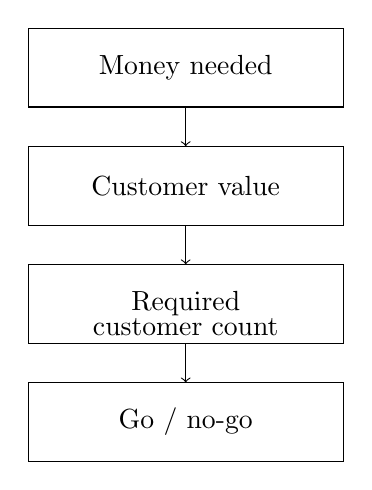
\begin{tikzpicture}[x=1cm,y=1cm]
\draw (0,0) rectangle (4,1);
\draw (0,-1.5) rectangle (4,-0.5);
\draw (0,-3) rectangle (4,-2);
\draw (0,-4.5) rectangle (4,-3.5);

\node at (2,0.5) {Money needed};
\node at (2,-1.0) {Customer value};
\node at (2,-2.5) {Required};
\node at (2,-2.8) {customer count};
\node at (2,-4.0) {Go / no-go};

\draw[->] (2,0) -- (2,-0.5);
\draw[->] (2,-1.5) -- (2,-2);
\draw[->] (2,-3) -- (2,-3.5);
\end{tikzpicture}
\caption{A narrow reconstruction of Jones's backward logic. We do not start from enthusiasm for the offering; we begin from the money requirement, convert that into customer value, and only then ask whether the resulting customer count is realistic.}
\end{figure}

\subsection{Question \& Answer}

The lecture pauses here around a small but decisive question: what mistake was made? The answer is subtle. We are very good at asking whether we \emph{could} do something. We are much less good at asking whether we \emph{should} do it. The arithmetic is introduced precisely to force that second question. A venture fails in many ways, but the terminal symptom is usually the same: it runs out of money, or it is on a path that will never produce any.

\section{Users, Payers, Champions, and What We Are Really Selling}

The lecture now complicates the example without abandoning it. The first market was schoolchildren. But the children are not the economic buyers. They are users. The likely payers are parents. That distinction alone matters, because it forces us to ask what the parent believes is being bought. A child may want fun, status, or escape from boredom. A parent may be buying discipline, an activity, or simply an experiment.

Jones then erases the first customer definition and starts over. What if the right customer is not the child at all, but the adult who used to play, who misses music, and who would pay to recover a piece of a lost self? Now the hourly rate can be higher, and the frequency higher as well. The transcript gives the endpoint directly:
\[
V_c\approx \$400 \text{ per month per customer.}
\]
On the same target income, that changes the count to
\begin{equation}
N\approx \frac{5{,}000}{400}=12.5,
\end{equation}
which Jones rounds in speech to ``about a dozen or so.'' The business itself has not been reinvented from nothing. The teaching is still there. What has changed is the customer definition, and with it the economics.

He then pushes the example further still, to older adults seeking not simply instruction but social life, companionship, purpose, and collaborative experience. This is a deep point in the lecture. The same visible product can be serving entirely different underlying demands. Jones says explicitly that if a business is to prosper, not merely limp along, it must discover what it is really selling.

\subsection{Question \& Answer}

The next question emerges naturally: who wins if I win? The immediate answer is the customer, but Jones does not let us stop there. Customers can become a sales force by talking to one another. Champions may recommend us. Economic buyers may be distinct from users. Adjacent collaborators may profit from our success.

His music-store example makes the structure concrete. A lapsed guitarist goes into a store for strings. The store clerk learns that he has no real opportunities to play and no clear path back to competence. The clerk can send him to the teacher. Then both parties win: the teacher gets a student, and the store eventually gets more sales in strings, instruments, and equipment. The lesson is not merely that referrals matter. It is that the venture sits inside a network of aligned incentives.

What, then, is being sold? The room offers ``romance,'' and Jones half accepts the answer before widening it. He is selling comfort, socialization, purpose, collaboration, and the excitement of shared performance. The guitar lesson is only the visible vehicle.

\section{The Non-Negotiable Requirement: Customers}

At this point Jones compresses the lecture into a checklist. What is broken? Who specifically wants a solution? Are there enough such people? Will they pay to solve the problem? How are they solving it now? Why is the proposed alternative compellingly better? Who exactly pays? These questions are easy to state and hard to answer, and he warns that neglecting them means driving into a hole.

He then states the investor's perspective with great bluntness. Investors, he says, usually want the answer to two questions: how will you make money, and how will I make money? But the first question dominates the second. If the venture cannot make money, the investor has no path to making money either. From that point of view there is only one non-negotiable requirement: customers.

This is the bridge between the toy model and the serious case study. Up to this point the lecture has been constructing a way of seeing. The next move is to show what happens when smart people do serious work and still get the customer wrong.

\section{Customer Discovery by Failure: The Regain Case}

Jones turns to a real venture from his own experience. He was running a highly profitable clinical nutrition division. The arithmetic of that business was excellent:
\begin{equation}
\text{cost per liter}\approx \$3,
\qquad
\text{sale price per liter}\approx \$70.
\end{equation}
The company had been doing roughly two hundred million dollars in annual revenue for years, but managed care threatened that profit pool. So he went searching for a new opportunity.

The opportunity seemed obvious. In the dialysis field there were roughly
\begin{equation}
400{,}000\ \text{patients}
\qquad \text{and} \qquad
2{,}300\ \text{dialysis centers},
\end{equation}
and patients commonly accumulated eight to twelve pounds of excess fluid between treatments. Yet the standard nutritional supplements were liquids. Jones and his colleagues designed a bar-like supplement, high in what the patients needed, low in what they should avoid, and without additional fluid. They named it \emph{Regain}. They ran a clinical trial, published it, and obtained the answer everyone wants to hear: it worked. It improved blood chemistries and extended lives.

Then came market research, and the market research seemed to confirm everything. Clinicians said they would recommend it to all of their patients, seven days a week, at about three dollars a bar. So the venture built its projections, prepared marketing materials, and launched.

The result was catastrophic. The transcript gives the comparison vividly:
\[
\$400{,}000 \text{ forecast} \qquad \text{versus} \qquad \$35{,}000 \text{ actual.}
\]
As a cleaned-up ratio,
\begin{equation}
\frac{35{,}000}{400{,}000}=0.0875<0.10.
\end{equation}
The launch came in at less than ten percent of forecast.

\subsection{Question \& Answer}

What went wrong? Jones lets the question hang, and the lecture answers it in layers.

First, the venture asked the wrong people. It surveyed clinicians, but clinicians were not the buyers and did not eat the product. When the company finally spoke to patients, it learned that many of them did not want it and could not afford it.

Second, it asked the wrong people about taste. In kidney failure the palate shifts, and a protein-heavy product can taste like spoiled meat. The team had judged the taste by its own palate rather than the patient's.

Third, it misunderstood motivation. The question that should have been asked was not simply whether kidney-failure patients \emph{needed} a better nutritional supplement. It was who these customers were. The transcript gives a rough decomposition:
\begin{equation}
33\%+44\%=77\%\approx \frac{3}{4}.
\end{equation}
That is, about three quarters of the target customers had arrived there through long-term mismanagement of diabetes or high blood pressure. Jones's conclusion is severe: a large fraction of the market had not been taking care of itself for years and was unlikely to start now.

Fourth, the company failed to recognize retailers as customers. A product that the end user does not demand, from a company the pharmacist does not know, has no obvious claim on shelf space.

The retailer's economics then appear. Shelf space is linear and already monetized. If a known product is removed and a new one inserted, the retailer sees lost revenue unless compensated. That compensation is the slotting fee. The number Jones gives is large enough to make the point unforgettable:
\begin{equation}
\$1{,}000{,}000 \text{ per quarter for CVS,}
\end{equation}
and that was only the beginning, with guaranteed-sale terms and chain-wide stocking requirements on top.

The failure, then, is not a single mistake. It is a chain of mistakes, each caused by an incorrect definition of the customer.

\section{Rebuilding the Business Around the Real Customer}

After other ventures and after a garbled transition in the transcript whose overall direction is nevertheless clear, Jones joins a new company in diabetes. Here the lecture reconstructs a business by starting much closer to the customer's actual experience.

The market is large:
\begin{equation}
10{,}000{,}000\ \text{diagnosed patients},
\qquad
4{,}000{,}000\ \text{insulin users}.
\end{equation}
The practical problem is not simply high blood glucose. It is the need to keep blood glucose within a tolerable band. During the day, disciplined patients can use small meals, small snacks, and regular insulin doses to moderate that band. At night the system breaks. People do not wake themselves repeatedly to snack and inject. Instead they take a large evening snack and a large insulin bolus and hope that the two will carry through the night.

The hope fails for a simple reason. The snack converts to glucose quickly, producing a higher spike without extending the time support. By the early hours of the morning the food is gone but the insulin is still acting. Jones identifies the dangerous interval schematically as
\begin{equation}
2\ \text{a.m.} \le t \le 6\ \text{a.m.}.
\end{equation}

\begin{figure}
\centering
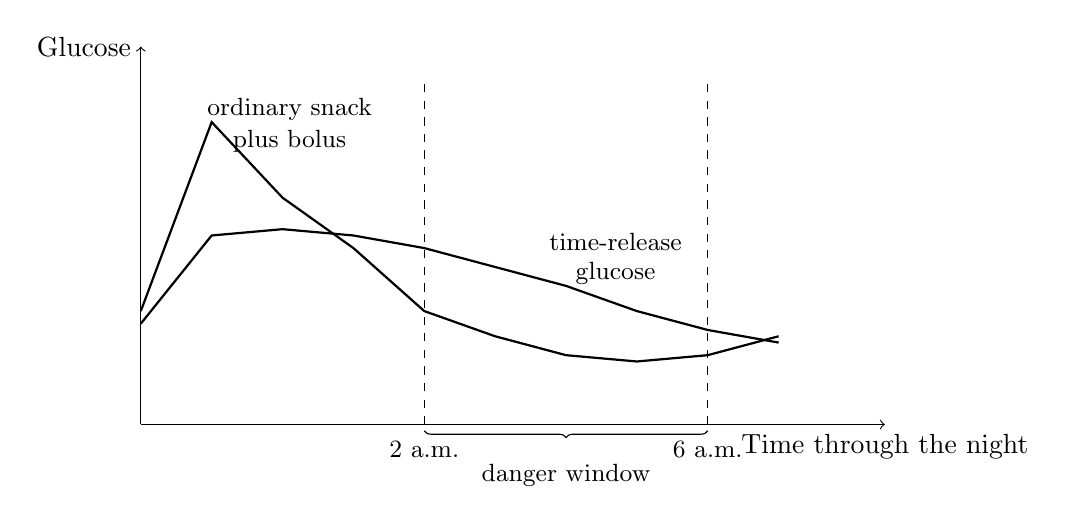
\begin{tikzpicture}[x=0.9cm,y=0.08cm]
\draw[->] (0,0) -- (10.5,0) node[below] {Time through the night};
\draw[->] (0,0) -- (0,60) node[left] {Glucose};

\draw[dashed] (4,0) -- (4,54);
\draw[dashed] (8,0) -- (8,54);
\node at (4,-4) {\small 2 a.m.};
\node at (8,-4) {\small 6 a.m.};

\draw[thick] plot coordinates {(0,18) (1,48) (2,36) (3,28) (4,18) (5,14) (6,11) (7,10) (8,11) (9,14)};
\draw[thick] plot coordinates {(0,16) (1,30) (2,31) (3,30) (4,28) (5,25) (6,22) (7,18) (8,15) (9,13)};

\node at (2.1,50) {\small ordinary snack};
\node at (2.1,45) {\small plus bolus};
\node at (6.7,29) {\small time-release};
\node at (6.7,24) {\small glucose};

\draw[decorate,decoration={brace,mirror}] (4,-1) -- (8,-1);
\node at (6,-8) {\small danger window};
\end{tikzpicture}
\caption{Schematic reconstruction from the transcript. The ordinary evening snack gives a higher early spike, but it does not carry glucose far enough into the dangerous overnight window. The redesigned product aims to release glucose more slowly across the night.}
\end{figure}

Focus groups now become decisive. Jones stops listening to the scientific explanation of the product and asks for fear. The answer is unforgettable: some patients sleep in a recliner because they fear dying in their sleep. That fear changes the venture. The company designs a product whose components convert to glucose at different rates and last through the night. The name given in the lecture is ``time-release glucose.''

A second practical redesign follows. This time the company involves not only clinicians but parents and patients in formulating the product. The dosage becomes simple and modular:
\begin{equation}
100\ \text{calories per unit},
\end{equation}
with scored portions that allow \(50\), \(100\), or \(150\) calories depending on the user.

\subsection{Question \& Answer}

Why would putting ``for diabetes'' on the label kill the business? Jones explicitly raises the question, because he originally thought the medical label would help. The customers teach him the opposite. They do not want to declare themselves as patients in public. ``I am not a diabetic,'' the imagined customer says; ``I am a banker, a lawyer, an entrepreneur.'' A product that looks like medicine signals sickness, frailty, and diminished professional standing. The same underlying chemistry must therefore be packaged as something an athlete might use, not as a visible badge of illness.

The lesson is subtle. Product efficacy is not enough. Identity enters the economics.

\section{Channels, Free Sales Forces, and Selling Customers to Retailers}

The same focus-group work also reveals something else: channel changes perceived value. When users are asked where they expect to buy the product and how much they expect to pay, the responses split into two piles:
\begin{equation}
\$0.49 \text{ in a grocery store},
\qquad
\$1.25 \text{ in a pharmacy.}
\end{equation}
The product is the same. The perceived value is not. Jones chooses the pharmacy channel.

From there the lecture becomes operational. The company looks for the subset of diabetes patients who actually spend time and money taking care of themselves. That search leads to certified diabetes educators, organized nationally and locally, and strongly motivated by one problem above all others: patient compliance. If they can recommend something that patients will actually use, they become an extraordinary unpaid sales force. Several thousand such professionals eventually work in that role for the company.

The sales model evolves in stages. At first the company sells directly in order to learn reorder behavior and infer usage rates. Then it uses advertising to generate calls, qualifies callers by asking about their insulin, sends samples, and follows up. In that process Jones emphasizes a small but important methodological point: open-ended questions are more informative than closed-ended ones. ``Did you like it?'' stops the conversation at yes or no. ``What did you think?'' opens it.

The empirical signal of demand is then read through volume:
\begin{align}
100 &\to 200 \to 300 \to 500 \quad \text{calls/day},\\
\text{reuse rate} &> 300 \quad \text{occasions/year}.
\end{align}
At that point the company is no longer guessing that it has found a need.

The pharmacy-entry tactic is equally concrete. A local manager often has a small-dollar purchase threshold below which corporate approval is unnecessary. Jones guesses that this threshold is about one hundred dollars, so the starter kit is priced just below it:
\begin{equation}
\$99.95<\$100.
\end{equation}
Risk is removed by promising a refund even if unsold stock is thrown away. Patients are then directed into the pharmacy, quick sell-through creates evidence, and reorders follow. In Jones's sharp formulation, the company has bought a group of customers and then sold those customers to the retailer.

A similar move is used with wholesalers. If the average large pharmacy carries about eight thousand SKUs, it does not want eight thousand invoices. Wholesalers therefore matter, and the company gets into their systems by seeding nearby pharmacies and guaranteeing the wholesaler its margin. Once reorder demand appears, the infrastructure is already in place.

The culminating retail anecdote makes the principle unmistakable. A chain buyer expects to spend all week extracting slotting fees from desperate vendors. Jones and his colleague arrive with no money to pay. Instead they put ten thousand existing customers on the table and ask a devastating question: when those customers ask which pharmacy carries the product, how should they answer? Silence does the work. The company gets in. What it had, as Jones says, was customers.

\section{Segment by Motivation, Not Demographics}

The lecture closes by extracting doctrine from the stories. One doctrine concerns benefits. Nobody wants the product as such. People want what the product does for them. Jones's example is vision correction: glasses, contact lenses, and LASIK are different products hired for the same job. The same principle governs everything in the chapter. Guitar lessons are not merely instruction. The nighttime glucose product is not merely glucose. Both are vehicles for something deeper.

The other doctrine concerns segmentation. Conventional marketing segments by geography, income, or gender. Jones argues that the entrepreneur, especially the undercapitalized entrepreneur, must segment by motivation. If we have a product that reduces the chance of a second heart attack, then the person who has just lived through the first one sits at the top of the motivational order. Family spillover comes next. Adjacent social groups come next. The broad public comes last:
\begin{equation}
\text{most motivated}
>
\text{related observers}
>
\text{adjacent social group}
>
\text{general public}.
\end{equation}
The broad public may be large, but for a startup it is often a graveyard. To change buying habits we need motivation, and Jones lists the strong forms of it plainly: pain, greed, fear, vanity. Virtue alone is a difficult sale.

His final quick story about the sleep product drives the point home once more. The company believed it was selling to overworked mothers. The real repeat buyers turned out to be marathon runners who valued the product because it improved recovery and therefore performance. A top-down demographic picture had obscured the actual job the product was hired to do.

The closing bridge to the next lecture is neat and practical. If one has not yet learned how to identify the customer and the benefit, one will not be able to pitch the business in three minutes, much less in thirty seconds or in three sentences.

\section{Summary}

The lecture begins with logistics and ends with pitch homework, but its center is a mathematical and strategic discipline. We begin at the end, with money needed. We divide by customer value to obtain customer count. We ask whether the resulting count is realistic. Then we sharpen the question: who uses the product, who pays, who recommends, who collaborates, and who else wins if we win?

The Regain failure shows what happens when those questions are answered badly. The Night Bite success shows what happens when the entrepreneur listens to fear, identity, channel behavior, and reorder evidence rather than to flattering abstractions. The final doctrine is severe but usable: do not chase everybody. Find the people who want the offering most, tell them about it, and take their order.